% !TEX root = ../MasterThesis.tex

\chapter{カロリメトリー技術} \label{sec:DeepLearning}
本章では、ILC実験およびEBES実験のために用いられるカロリメトリー技術について述べる。2.1節ではカロリメトリーの基本的な動作原理となる物理現象について説明する。2.2節ではカロリメータを用いた測定技術について述べる。2.3節ではカロリメータにおいてジェットエネルギー分解能向上のためのアルゴリズムの一つであるParticle Flow Algorithm (PFA)について説明する。
\section{カロリメトリーに関する物理現象}
素粒子実験で検出対象となる粒子は、検出器との相互作用を生じさせることにより、その位置やエネルギーなどの情報を測定することが可能となる。これまでに行われてきた理論計算や実験などによって、粒子の検出器に対する応答が明らかとなっている。
\subsection{荷電粒子と物質の相互作用}
荷電粒子は物質中では原子内に存在する原子核や電子と電磁相互作用を行う。主には励起や電離といった反応が起こり、入射してきた荷電粒子は徐々に速度を落としていく。Bethe-Blochの行った計算によると、荷電粒子が物質中で落とす単位長あたりのエネルギー損失は
\begin{equation}
-\frac{dE}{dx} = \frac{4\pi \alpha^2 \hbar^2 q^2 n_e}{m_e\beta^2}\left[\ln\left(\frac{2m_ec^2 \beta^2\gamma^2}{I}\right)-\beta^2-\frac{\delta(\gamma)}{2}\right]
\end{equation}

\begin{table}[H]
	\begin{center}
		\begin{tabular}{ll}
			$\alpha$ : 微細構造定数($\simeq 1/137$) & $\hbar$ : ディラック定数\\
			$n_e$ = $\rho N_A Z/A$ : 電子密度& $q$ : 入射粒子の持つ電荷 \\
			$N_A$ : アボガドロ数 & $\beta = v / c$ ($v$ : 入射粒子の速度、$c$ : 光速) \\
			$Z$ : 吸収体の原子番号 & $\gamma$ = $(1-\beta^2)^{-1/2}$ \\
			$A$ : 吸収体の質量数 & $I$ : イオン化ポテンシャル \\
			\multicolumn{2}{l}{$\delta$ : 吸収体原子内の電子による電場の遮蔽効果のパラメータ} \\
		\end{tabular}
	\end{center}
\end{table}

となる。このBethe-Blochの式に基づく入射粒子のエネルギーに対するエネルギー損失の大きさを示したグラフを図\ref{Bethe}に示す\cite{PDG_Interaction}。
\begin{figure}[H]
	\begin{center}
		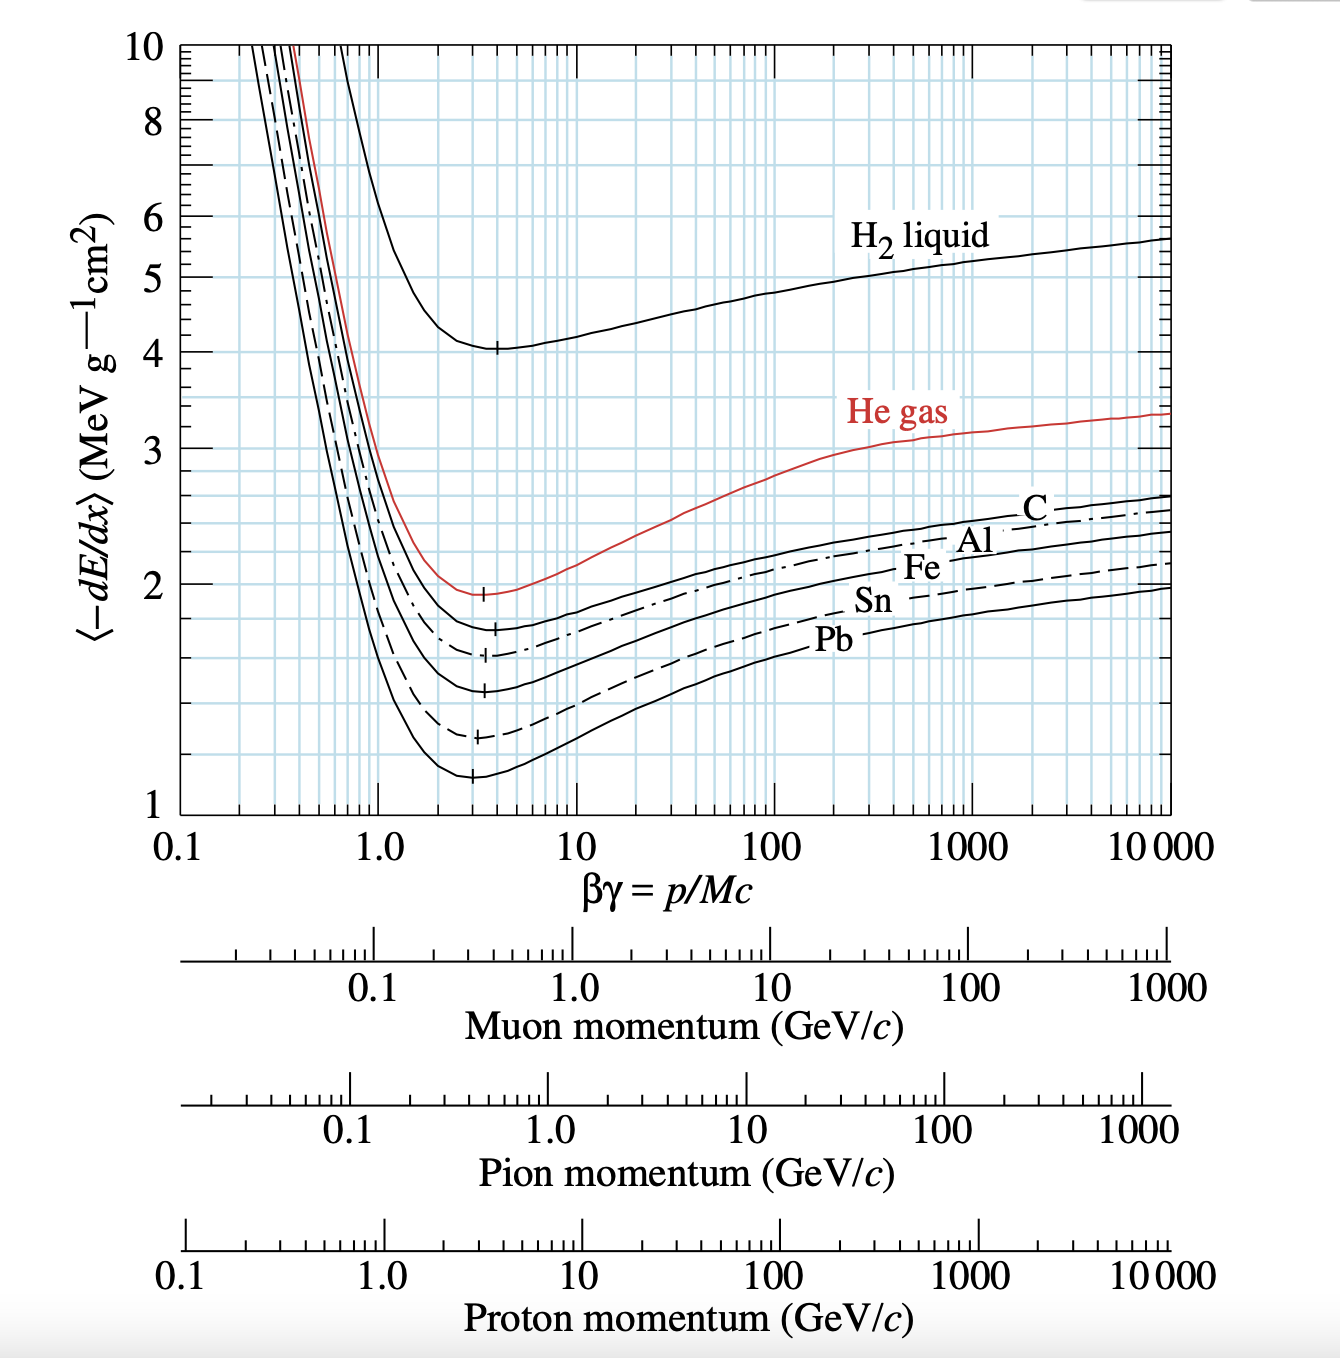
\includegraphics[width=370pt]{./Figure/EcalDetector/Bethe.png}
		\caption[Bethe-Blochの式に基づくエネルギー損失]{Bethe-Blochの式に基づくエネルギー損失}
		\label{Bethe}
	\end{center}
\end{figure}


この図から分かるように、エネルギー損失は特定の運動量において最小となり、それより高い運動量ではゆるやかに上昇する。エネルギー損失が最小となる運動量付近にある粒子をMIP (Minimum Ionizing Particle)と呼ぶ。

\subsection{光子と物質の相互作用}
光子は電荷を持たないため、荷電粒子とは異なる相互作用を引き起こす。主として生じる相互作用は、光電効果、コンプトン散乱、電子対生成の3つである。

\begin{description}
\item 光電効果:

エネルギーの小さい光子が物質中に入射すると、原子内の電子が光子のエネルギーを全て吸収し、吸収したエネルギーが束縛エネルギー以上であればその電子は物質外へと放出される。この現象を光電効果と呼ぶ。相対論的速度に近づくほど光子の十分にエネルギーが大きいとき、その断面積は
\begin{equation}
\Phi_{\mathrm{photo}} = 4\alpha^4 \sqrt{2} Z^5 \phi_0 \left(\frac{m_ec^2}{h\nu}\right)^{\frac{7}{2}}
\end{equation}
と表される\cite{HEPDetector}。ただし、$m_e$は電子質量、$\phi_0 = \frac{8\pi r_e^2}{3}=6.651\times 10^{-25}\SI{}{cm^2}$($r_e$は古典電子半径)は古典的なトムソン散乱の断面積である。
	
	
\item コンプトン散乱:

光子のエネルギーがある程度大きくなると、電子が光電効果による全てのエネルギーを吸収しきれなくなり、電子と光子の散乱現象が生じる。これがコンプトン散乱である。コンプトン散乱の断面積は次のクライン-仁科の公式
\begin{equation}
\frac{d\sigma_{\mathrm{compton}}}{d\Omega}=\frac{r_e^2}{2}\frac{1}{[1+\gamma(1-\cos\theta)]^2}\left(1+\cos^2\theta+\frac{\gamma^2(1-\cos\theta)^2}{1+\gamma(1-\cos\theta)}\right)
\end{equation}
により記述されることが知られている。

\item 電子対生成:

光子のエネルギーがおよそ$\SI{1.02}{MeV}$以上になると、光子が物質中の原子核と相互作用することにより生じる電子対生成現象が起こり始める。これは光子のエネルギーが電子および陽電子の質量へと転換されることにより電子陽電子ペアが生じる現象である。カロリメータ中における高エネルギー反応においてはこの電子対生成反応が主要な寄与を示し、後述する電磁シャワーを発生させる一因となる。この断面積は近似的に
\begin{equation}
\sigma_{\mathrm{pair}} \approx \frac{7}{9}\frac{A}{N_AX_0}
\end{equation}
で表される。ただし、$A$は物質の質量数、$N_A$はアボガドロ数、$X_0$は放射長である。ここで、放射長$X_0$は
\begin{equation}
X_0= 4\left(\frac{\hbar}{mc}\right)^2Z(Z+1)\alpha^3n_a\ln\left(\frac{183}{Z^{1/3}}\right)
\end{equation}
と表され、この長さは荷電粒子のエネルギーが$1/e$に減少するまでに物質中を通過する平均距離を示している。

\end{description}
	
これらの3つの現象の断面積は、光子のエネルギーおよび媒質によって大きな違いが生じる。炭素および鉛に対して、照射した光子のエネルギーごとに各反応の断面積を示したものを図\ref{photonInteract}に示す。

\begin{figure}[H]
	\begin{center}
		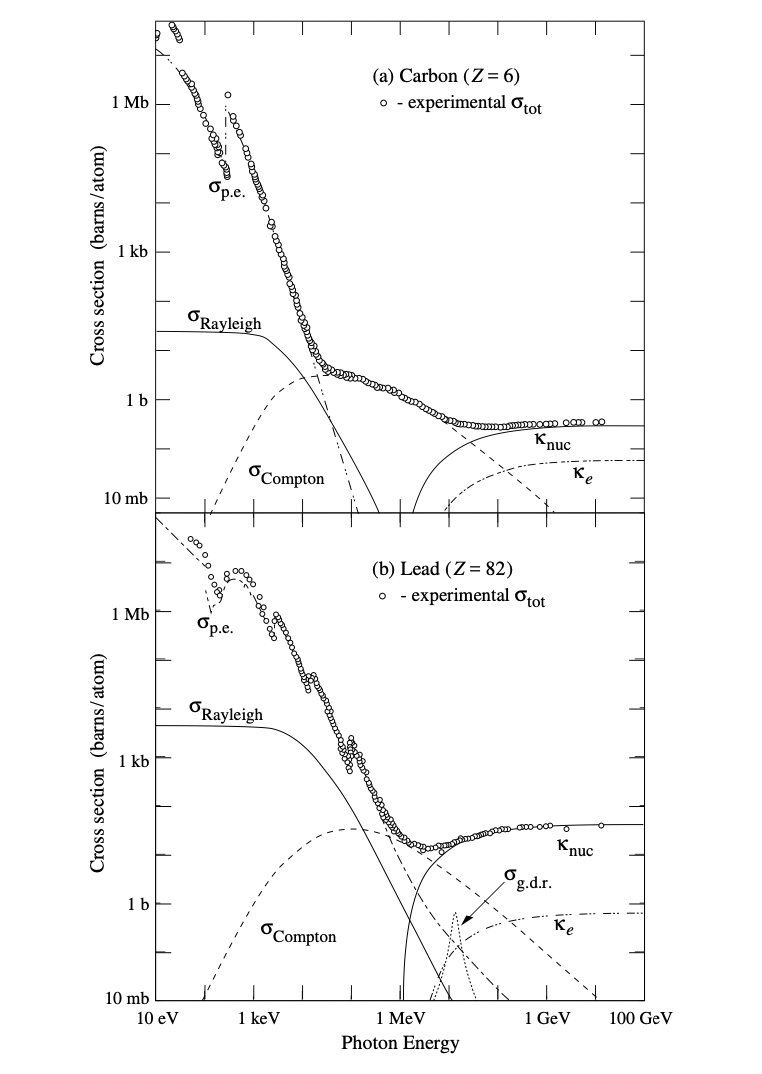
\includegraphics[width=370pt]{./Figure/EcalDetector/PhotonInteract.png}
		\caption[光子のエネルギーに対する相互作用断面積]{炭素C、鉛Pbに入射した時の光子のエネルギーに対する相互作用断面積\cite{PDG_Interaction}。}
		\label{photonInteract}
	\end{center}
\end{figure}


\subsection{制動放射}
荷電粒子は前述の通りイオン化や光電効果などによってエネルギーを失う他、制動放射(bremsstrahlung)と呼ばれる、主に原子核との相互作用によって光子が放出される現象とともに大きなエネルギー損失が生じる。この反応は電子や陽電子に対して主要なエネルギー損失となりうる。

この反応による平均のエネルギー損失は
\begin{equation}
-\frac{dE}{dx} = \frac{E}{X_0}
\end{equation}
と表される。

制動放射によって失われる放射長あたりのエネルギー損失と電子のエネルギーが等しくなる時のエネルギーを臨界エネルギー(Critical Energy)と呼ぶ。この時のエネルギー損失はエネルギーを$E$とすると、
\begin{equation}
\left|\frac{dE}{dx}\right|_{\mathrm{brems}}\approx  \frac{E}{X_0}
\end{equation}
となる。

\subsection{チェレンコフ光}
荷電粒子が物質中を通過するとき、同じ媒質中を通過する光よりも速く運動する場合、チェレンコフ光と呼ばれる光が発生する。
この速度$v_{\mathrm{particle}}$は光速$c$、粒子の速度を$\beta c$、生じたチェレンコフ光の数を$n$とすると、
\begin{equation}
\beta c = v_{\mathrm{particle}} > c/n
\end{equation}
で与えられ、生じるチェレンコフ光により生じる円錐の開き角$\theta_C$は
\begin{equation}
\cos\theta_C=\frac{1}{\beta n(\omega)}
\end{equation}


この時放出される光子の数はチェレンコフ光の波長$\lambda$および単位長さ$x$あたり、

\begin{equation}
\frac{d^2 N}{d\lambda dx}=\frac{2\pi z^2\alpha}{\lambda^2}\left(1-\frac{1}{\beta^2n^2(\lambda)}\right)
\end{equation}

と表される。ただし、荷電粒子の電荷$z$、微細構造定数を$\alpha$、$n(\omega)=1/(\beta \cos\theta_C)$である。
チェレンコフ光の数は粒子の数および飛程にほぼ比例している。

%%%%%%%%%%%%%%%%%%%%%%%%%%%%%%%%%%%%%%%%%%%%%%%%%%%%%%%%%%%%%%%%
\begin{comment}
このチェレンコフ光により荷電粒子が失うエネルギーは、荷電粒子の電荷を$z$、微細構造定数を$\alpha$、光速$c$、粒子の速度を$\beta c$、チェレンコフ光の波長を$\omega$として、
\begin{equation}
-\frac{dE}{dx} = z^2 \frac{\alpha \hbar}{c} \int\omega d\omega\left(\1-\frac{1}{\beta^2n^2(\omega)}\right)
\end{equation}
と表される。
\end{comment}
%%%%%%%%%%%%%%%%%%%%%%%%%%%%%%%%%%%%%%%%%%%%%%%%%%%%%%%%%%%%%%%%

\subsection{電磁シャワーおよびハドロンシャワー}
十分に大きなエネルギーを持った荷電粒子および中性粒子が物質中に入射すると、電磁シャワーやハドロンシャワーのような特徴的な現象が生じる。

電磁シャワーは上で述べた電子対生成が関与している。光子が大きなエネルギーを持っている場合、その光子が変換されて生じた電子および陽電子もまた大きな運動エネルギーを持って放出される。この場合、電子が制動放射を起こすことにより新たな光子を生成することになる。この結果、エネルギーが十分小さくなるまで電子陽電子対生成と制動放射が繰り返し引き起こされる。

シャワーの大きさは、物質の厚さと放射長に依存する。シャワー内に含まれる合計の粒子数(光子や電子、陽電子)$N$は物質の厚さが放射長の$t$倍であるとすると、
\[
N = 2^t
\]
と表される。

%%%%%%%%%%%%%%%%%%%%%%%%%%%%%%%%%%%%%%%%%%%%%%%%%%%%%%
\begin{comment}
この時、生じるカスケードの最大厚み$t_{max}$は入射光子のエネルギーを$E_0$、臨界エネルギー$E_c$に対して、
\[
E(t_{\mathrm{max}}) = \frac{E_0}{2^{t_{\mathrm{max}}}}=E_c
\]
より、
\[
t_{\mathrm{max}} = \frac{\ln{\frac{E_0}{E_C}}}{\ln{2}}
\]
となる。
\end{comment}
%%%%%%%%%%%%%%%%%%%%%%%%%%%%%%%%%%%%%%%%%%%%%%%%%%%%%%


電磁シャワーの90\%のエネルギー損失が収まるように円筒領域を考えたときに、その円筒の半径をMoliere 半径と呼ぶ。Moliere 半径$R_M$は臨界エネルギーを$E_C$、放射長を$X_0$とすると、
\begin{equation}
R_M = X_0 \frac{21\ [\SI{}{MeV}]}{E_C}
\end{equation}
と表される。シャワーの全エネルギーのうち、$3.5R_M$には99\%のエネルギーが吸収されている。

ハドロンシャワーは荷電ハドロンおよび中性ハドロンが物質中に入射することで生じる。ハドロンシャワーは非常に複雑な過程が混在する。入射してきた高エネルギーハドロンは物質中の原子核および電子と非弾性散乱を行い、二次的な相対論的エネルギーハドロンの生成や$\SI{100}{MeV}$程度の核破砕核の放出、ハドロンによる原子核の破壊などが生じる。これらの核反応の連鎖によりシャワーを発生する。
一方、これらの相互作用の生成物に含まれる$\pi_0$中間子の発生は$\pi_0$から崩壊した$\gamma$線による電磁気的相互作用の寄与を伴う。この電磁シャワーはハドロンシャワーと比較して同じエネルギー損失あたりの発生粒子数が異なるので、大きな誤差要因となりうる。この影響を低減させるためにCompensationやDual-readoutといった検出器技術が開発されている。Compensationでは、電磁シャワーもハドロンシャワーもエネルギーあたり同じ信号強度になるようにしたり、検出器ハードウェアを工夫したりすることによって電磁成分とハドロン成分の差を小さくする技術である。その技術の一つであるDual-readout技術は荷電ハドロンおよび電磁シャワーをシンチレーション光とチェレンコフ光による2重読み出しによって測定を行い、それぞれの寄与を別々に測定するために開発されている。



\section{カロリメータ技術}
カロリメータは入射してきた光子や荷電粒子などによって生成されたシャワーをカロリメータ内で吸収することにより入射粒子のエネルギーを測定する。
この項では、カロリメータ検出器による粒子検出の原理について、説明を行う。2.2.1節および2.2.1節では全吸収カロリメータとそのうちの一種である鉛ガラス検出器について述べる。2.2.3節ではもう一つのカロリメータであるサンプリング型カロリメータについて取り上げる。

\subsection{全吸収型カロリメータ}
全吸収型カロリメータは検出器全体が吸収体となっており、電子や光子の入射で発生する電磁シャワーによるシンチレーション光やチェレンコフ光\cite{PDG_Cal}を検出し、光電子増倍菅(Photomultiplier Tube, PMT)により増幅する。これらの検出器には主に原子番号の大きな鉛ガラスやクリスタルが用いられ、一例として$\textrm{BaF}_2$やCsI(Tl)、LYSOなどが用いられる。これらの検出器はエネルギー分解能が高く、特に低エネルギーの粒子を精度良く測定するのに向いているが、これらの物質は微細分割のコストが高く、またエネルギー較正が難しい点が短所として挙げられる。

\subsection{鉛ガラス検出器}
鉛ガラスチェレンコフ検出器は入射した荷電粒子や光子の検出およびそのエネルギー測定を行うための検出器である。鉛ガラス中で電磁シャワーから放出される電磁シャワーに含まれる電子の一部は媒質中での光速を超え、チェレンコフ光を発生させる。%鉛ガラス検出器の表面を反射材に覆うことで、チェレンコフ光は内部で反射し検出器の一面に取り付けられたPMTへと集光される。
チェレンコフ光は空気と鉛ガラスの境界での全反射に加えて、表面を反射材で覆うことで内部で反射し、検出器の一面に取り付けられたPMTへと集光される。
発生するチェレンコフ光の光子数は入射した荷電粒子の数および飛程にほとんど比例し、電磁シャワーではエネルギーと粒子数が概ね比例するため、結果としてPMTにおいて光から変換された電気信号を測定することで荷電粒子のエネルギーを決定することが可能である。PMTは外部からの光に敏感であり、光の漏れがあると信号が大きくなるため、遮光を十分に行う必要がある。

今回EBES実験のために使用する鉛ガラス検出器はTRISTAN/TOPAZ実験で使用された、ビーム軸に対する面積が$150\times\SI{150}{mm^2}$、奥行きが$\SI{30}{cm}$の検出器である\cite{LeadGlass}。概形を図\ref{PbO}に示す。放射長に対する奥行きは$17.7X_0$に対応しており、検出器を構成する成分は55\%がPbO、45\%が$\textrm{SiO}_2$となっている。この検出器に対して光電子増倍菅を接続し、光検出を行う。

\begin{figure}[H]
	\begin{center}
		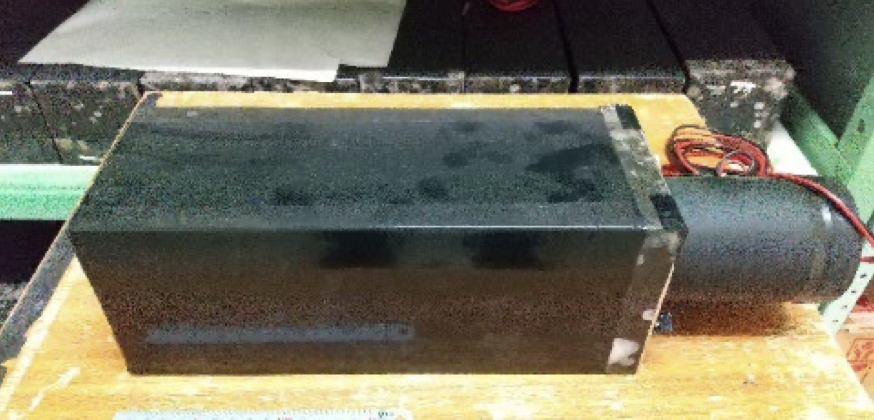
\includegraphics[width=370pt]{./Figure/EcalDetector/PbO.png}
		\caption[EBES実験に使用する鉛ガラス検出器]{EBES実験に使用する鉛ガラス検出器。}
		\label{PbO}
	\end{center}
\end{figure}


\subsection{サンプリング型カロリメータ}
サンプリング型カロリメータは吸収体と検出層を別々に構成することによって、微細化したカロリメータを構成することができる。光子や電子が入射すると、吸収体によって電磁シャワーへと変換され、シャワーによって運搬されたエネルギーが検出層において検出される。カロリメータに入射してきた粒子の全エネルギーに対する検出層の吸収エネルギーはサンプリング率と呼ばれ、サンプリング型カロリメータの性能を示す指標の一つとなっている。検出層には主に半導体やシンチレーター、ガスイオン検出器が用いられる一方、吸収層にはタングステンや鉛、鉄などといった原子番号の大きな金属が用いられる。サンプリング型カロリメータの構造については複数のタイプが考えられ、吸収層と検出層のプレートを交互に重ねたサンドイッチ構造のものやファイバーのような検出層を吸収体の中に埋め込むものなどがある。吸収層の間に挿入された検出層の多くのチャンネルから信号を読み出す方法が問題となり得るが、一つの解決策として読み出し回路を検出器内に挟み込んで読み出しを行なっている。

\subsection{SiW電磁カロリメータ}
ILDに使用される電磁カロリメータの一つとして、SiW電磁カロリメータ(SiW ECAL)が開発されている。その全体像を図\ref{SiW Ecal}に示す。このカロリメータはシリコン検出層とタングステン吸収層を交互に30層組み合わせたサンドイッチ構造を持つサンプリングカロリメータである。この節でそれぞれの特徴について述べた後、2.2.3節でシリコン検出層から送信されてきた信号を統括する読み出し回路について説明する。

\begin{figure}[H]
	\begin{center}
		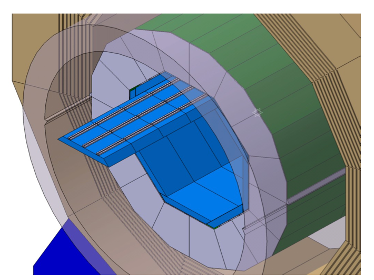
\includegraphics[width=250pt]{./Figure/EcalDetector/ILD_det_3D.png}
		\caption[ILD・ECALの全体像]{ILD ECALの全体像。青色で示されているのがECAL、緑色で示されているのがHCALである。}
		\label{SiW Ecal}
	\end{center}
\end{figure}


\begin{itemize}
\item シリコン検出層

ILDにおける電磁カロリメータは後に説明するParticle Flow Algorithm(PFA)を実行するために十分に微細化されている必要がある。そのためシリコン検出層は$1.0\times10^{8}$チャンネルまで微細化された検出器として開発が進められている。SiWECALを図\ref{ECAL_layer}に示す。それぞれの層にはFEVボードと呼ばれる電子回路が搭載されており、1枚のFEVボードには4枚のシリコンパッドが使用されている。

\begin{figure}[H]
	\begin{center}
		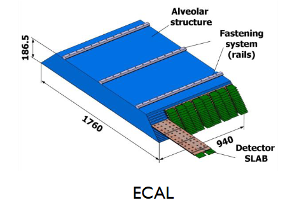
\includegraphics[width=250pt]{./Figure/EcalDetector/ECAL_layer.png}
		\caption[SiWECAL]{SiWECALの模式図。図中にはFEVボードが示されている。}
		\label{ECAL_layer}
	\end{center}
\end{figure}

シリコンは半導体の一種であり、荷電粒子検出器の原料として用いることができる。ここではそのうち、PN接合型と呼ばれる検出器の動作原理について述べる。半導体には多く存在しているキャリア電荷が正か負かによってP型およびN型の2種類に分けることができ、PN接合型の検出器はこの2種類の半導体素子を組み合わせることによって製造される。二つの半導体素子の中間には、正キャリア(正孔)と負キャリア(電子)が結合することにより空乏層と呼ばれる電気的に中性の領域が生じる。この空乏層に荷電粒子が入射すると、光電効果やコンプトン散乱により電子がP型半導体側へと放出される。一方、もともと電子が存在していた部分は負電荷欠乏となるため、電気的に正のキャリアが存在していると考えられ、この正キャリアはN型半導体へと移動する。この電子および正孔のペアを電子正孔対と呼ぶ。以上の電子正孔対の移動により、シリコン検出器内に電流が流れ、この電流を検出することによりガンマ線の測定を行うことが可能となる。一方、荷電粒子の場合は空乏層に入射するとイオン化が生じることにより電子の移動が起こり、以下ガンマ線の場合と同様にして荷電粒子の検出を行う。また、シリコン素子の両側に外部から電圧を印加すると検出領域である空乏層が広がるため、有感領域を拡大することができる。電圧を上げるほど空乏層の厚みは増加し、素子全体が空乏層となることを完全空乏化と呼ぶ。


現在のプロトタイプでは、1枚のパッドは大きさが$180\times \SI{180}{mm^2}$、厚さが$320-\SI{650}{\mu m}$となっている。シリコンパッドを4枚組み合わせることでActive Signal Units (ASU)が構成され、それぞれのシリコンパッドは大きさが$90\times \SI{90}{mm^2}$となっている。1枚のシリコンパッドにはさらに256個のチャンネルがあり、1チャンネルのピクセルサイズは$5.5\times\SI{5.5}{mm^2}$である。1枚のFEVボードを図\ref{FEV}に示す。

\begin{figure}[b]
	\begin{center}
		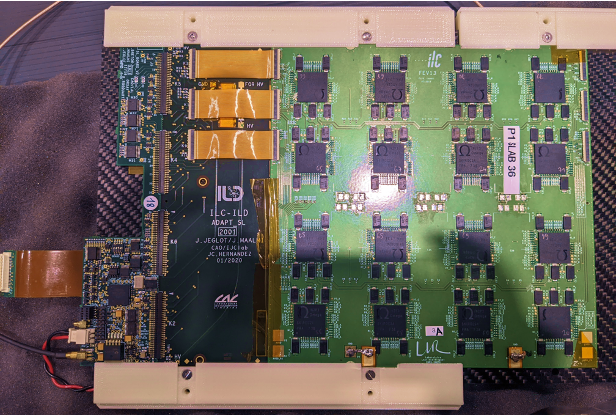
\includegraphics[width=250pt]{./Figure/EcalDetector/ECAL_board.png}
		\caption[FEVボード]{FEVボードの写真。16枚のASICチップとSLボードが搭載されている。}
		\label{FEV}
	\end{center}
\end{figure}

それぞれのASUには読み出しのためのSKIROC2 (A)と呼ばれるApplication Specific Integrated Circuits (ASICs)が備え付けられている。

\item タングステン吸収層

それぞれのシリコン検出層の間にはタングステン吸収層が挿入されており、カロリメータ全体で30枚となる。一枚の厚さは$\SI{2.1}{mm}$もしくは$\SI{4.2}{mm}$であり、厚さの合計は$24X_0$となる。タングステンを吸収層に選んだ理由としては、相互作用長が放射長のおよそ28倍となるため光子とハドロンの識別が優れている点や、$R_M$が小さくなる点が挙げられる。
\end{itemize}


%\subsection{シリコン検出器の動作原理}
%シリコンは半導体の一種であり、ガンマ線および荷電粒子検出器の原料として用いることができる。ここではそのうち、PN接合型と呼ばれる検出器の動作原理について述べる。半導体には多く存在しているキャリア電荷が正か負かによってP型およびN型の2種類に分けることができ、PN接合型の検出器はこの2種類の半導体素子を組み合わせることによって製造される。二つの半導体素子の中間には、正キャリアと負キャリアが結合することにより空亡層と呼ばれる電気的に中性の領域が生じる。この空乏層にガンマ線が入射すると、光電効果やコンプトン散乱により電子がP型半導体側へと放出される。一方、もともと電子が存在していた部分は負電荷欠乏となるため、電気的に正のキャリア(正孔)が存在していると考えられ、この正キャリアはN型半導体へと移動する。この電子および正孔のペアを電子正孔対と呼ぶ。以上の電子正孔対の移動により、シリコン検出器内に電流が流れ、この電流を検出することによりガンマ線の測定を行うことが可能となる。一方、荷電粒子の場合は空乏層に入射するとイオン化が生じることにより電子の移動が起こり、以下ガンマ線の場合と同様にして荷電粒子の検出を行う。特にシリコン素子の両側に外部から電圧を印加すると検出領域である空乏層が広がるため、有感領域を拡大することができる。電圧を上げるほど空乏層の厚みは増加し、素子全体が空乏層となることを完全空乏化と呼ぶ。

%\subsection{シンチレーション光}

\section{カロリメトリーにおけるPFAの利用}
ジェットエネルギー分解能を向上させるための技術として、PFAと呼ばれる手法があり、ILC実験ではこの手法を採用することで精度良くジェットエネルギー測定を行う。2.3.1節ではPFAの概要を説明する。2.3.2節ではPFAがどのようにILCのソフトウェアに組み込まれているかを説明するために、ILCにおけるソフトウェアエコシステムの全体像について述べる。2.3.3ではILCにおけるPFAアルゴリズムとして利用されているPandoraPFAについてその概要を述べる。2.3.4ではPandoraPFAを利用した際の粒子識別性能およびジェットエネルギー分解能を確認する。

\subsection{PFA}
電子陽電子ビームの衝突によって高エネルギーのクォークペアが生じると、クォークは単独では存在できないため強い相互作用による破砕化(フラグメンテーション)によって2つのジェットと呼ばれる粒子朿が形成される。これらのジェットは複数の荷電ハドロンや中性ハドロンを伴って飛跡検出器を通過した後、カロリメータへと入射する。

PFAは光子、荷電粒子、中性ハドロンのそれぞれを別々の検出器によって検出することによりジェットエネルギー分解能を向上させるための手法である。PFAを使う測定器では、光子は電磁カロリメータ、荷電粒子は飛跡検出器、中性ハドロンはハドロンカロリメータで検出が行われる。それぞれのジェットが持つエネルギーの全エネルギーに対する割合は荷電粒子がおよそ60\%、光子がおよそ30\%、中性ハドロンがおよそ10\%となる。荷電粒子(ほとんどがハドロンである)をハドロンカロリメータではなく飛跡検出器で測ることで、ジェットエネルギー分解能が大幅に向上する。ILC検出器における各粒子の分離の様子を図\ref{PFA_ILC}に示す。検出器は内側から、飛跡検出器、ECAL、HCALを示している。
\begin{figure}[H]
	\begin{center}
		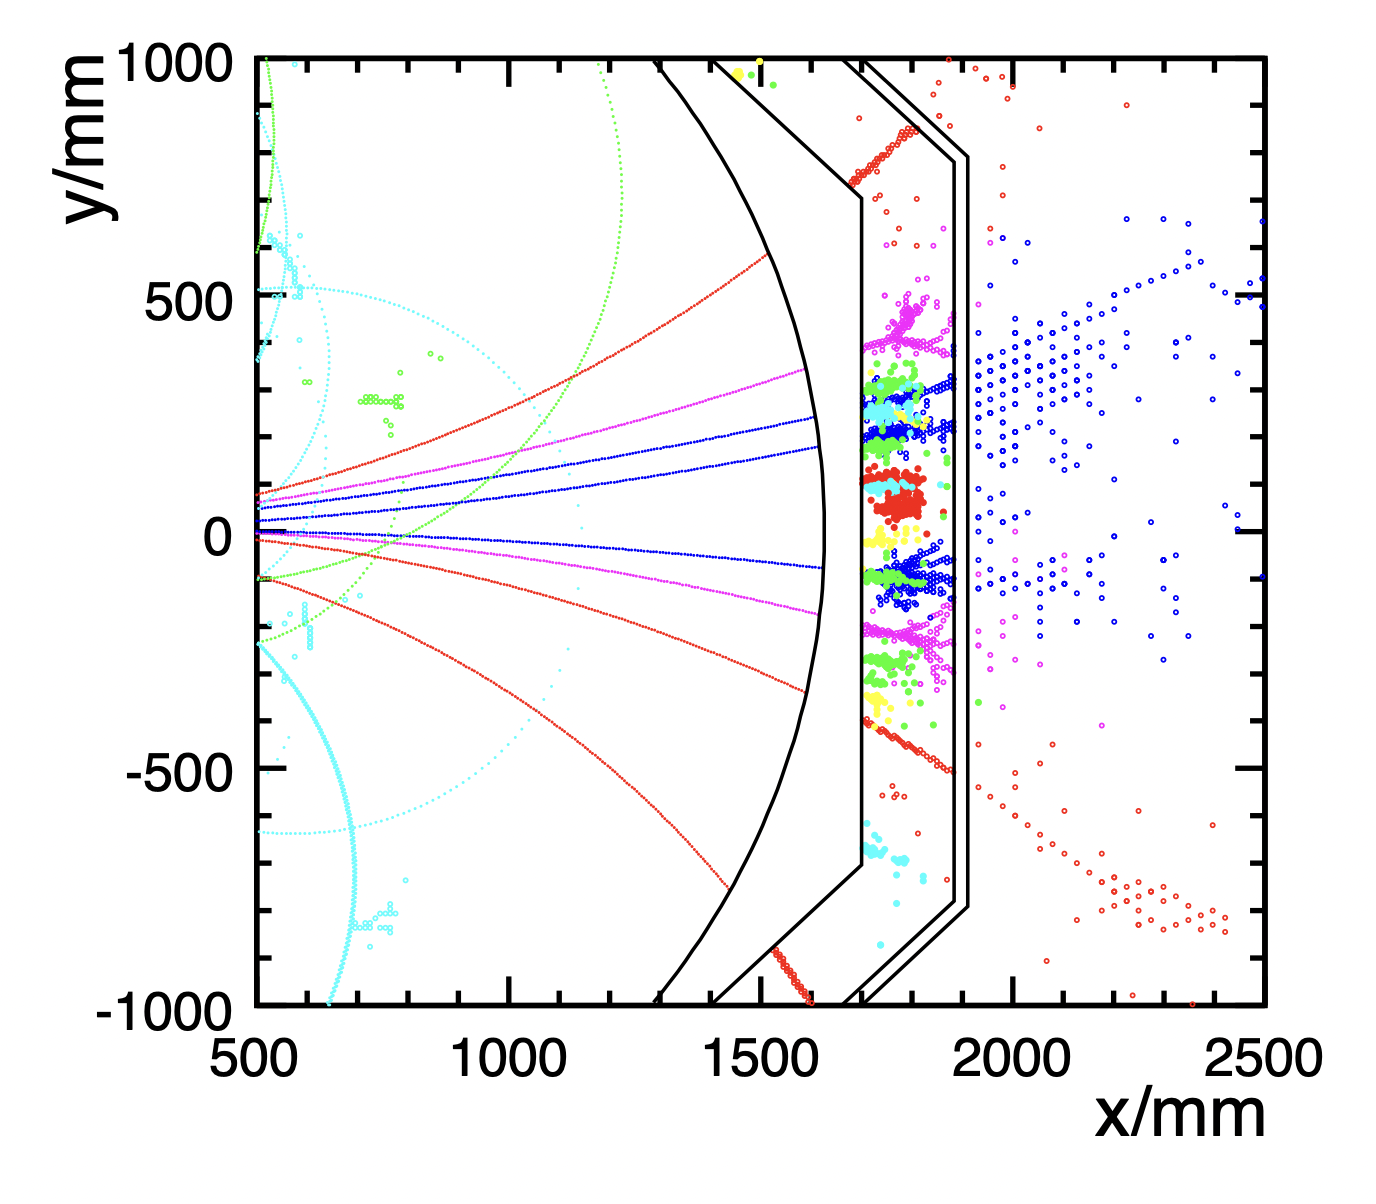
\includegraphics[width=370pt]{./Figure/EcalDetector/PFA_ILC.png}
		\caption[ILCにおける粒子識別の様子]{ILCにおける粒子識別の様子。異なる種類の粒子が異なる色によって識別されている。}
		\label{PFA_ILC}
	\end{center}
\end{figure}



各粒子を分離するために、検出器は非常に微細化されている必要がある。そのため、ILDに備えられる検出器は非常に多くのチャンネルを持った検出器となっている。

\begin{comment}
\subsection{iLCSoft}
ILCは現在計画段階にあり、検出器のジオメトリの設計や、目的とする新物理探索などについて決定するためにはソフトウェア技術が欠かせない。iLCSoftは線形加速器におけるシミュレーションや飛跡再構成、物理解析を行うためのソフトウェアエコシステムであり、LCIOやMarlin、DD4hepといったフレームワークを含んでいる。

iLCSoftを含むILC Softwareのワークフローを図\ref{iLCSoft_workflow}\cite{ILCSoftware}に示す。

まず、whizardやphyssimなどを用いて、目的とするイベントの生成が行われる。生成されたイベントはstdhepやlcioと呼ばれるフォーマットで保存される。これらのイベントを入力として、iLCSoftは検出器シミュレーションやイベント再構成を行う。検出器シミュレーションはGeant4をベースにしたDD4Simによって、またイベント再構成はMarlin(Modular Analysis \& Reconstruction for the LINear collider)と呼ばれるアプリケーションによって実行される。Marlinの中に含まれるのがジェットエネルギー再構成のためのPandoraPFAや飛跡再構成のためのTracking、崩壊点検出のためのLCFIPlusなどである。これらの情報がDSTMergedによって統合され、最終的にRootやPythonなどによる解析が行われる。

\begin{figure}[H]
	\begin{center}
		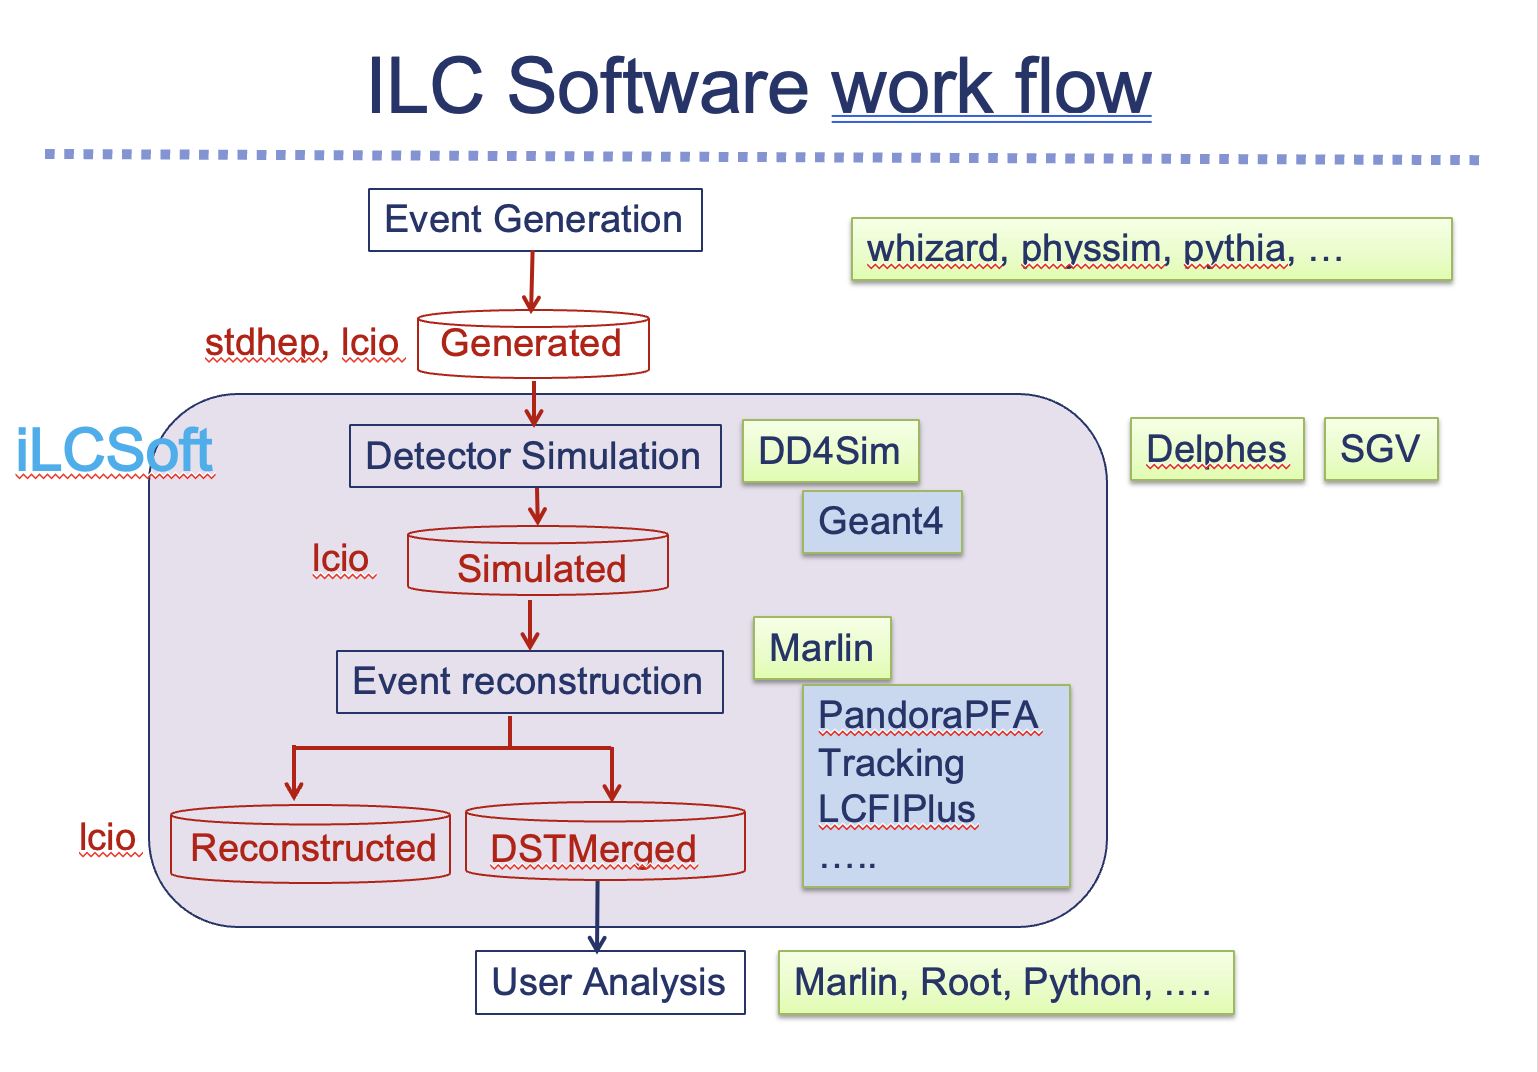
\includegraphics[width=370pt]{./Figure/EcalDetector/workflow.png}
		\caption[ILC Software のワークフロー]{ILC Software のワークフロー}
		\label{iLCSoft_workflow}
	\end{center}
\end{figure}
\end{comment}

\subsection{PandoraPFA}
PandoraPFA~\cite{PandoraPFA}はILCへ向けて開発されたPFAのためのソフトウェアである。PandoraPFAによるカロリメータクラスタリングおよび再構成はカロリメータにおけるヒットの情報やTPCにおける飛跡情報などを元にして行われる。一連の流れを示した図\ref{PandoraPFA}を示す。飛跡の情報はカロリメータのクラスタとマッチングするために用いられる。。カロリメータヒットの情報は3次元空間における位置、エネルギー損失、ECALおよびHCALのレイヤー番号を入力として使用する。入力されたヒットのうち、エネルギー損失が一定のヒットは削減され、その他のヒットはECALかHCALかで異なる較正係数を用いてエネルギー較正が行われる。%次に、ヒットのタグ付けに移る。あるヒットの周囲のヒットが基準値よりも低く、同じ層の隣接したセルでヒットが必要以上に存在していない場合に、そのヒットがMIPであると推定される。
PandoraPFAにおけるクラスタリングは各レイヤーごとのヒットから計算されるコーン角に基づいて計算される。まず、ビーム衝突点に近いレイヤーから順にカロリメータのヒット$i$がひとつ前のレイヤーのヒット$j$と比較される。
%二つのヒットの距離$\mathbf{r}_{ij}$とひとつ前のレイヤーのヒットから次のレイヤーのヒットへの向きを持つ単位ベクトル$\hat{\mathbf{u}}$を用いて、$d_\parallel = \mathbf{r}_{ij}\cdot \hat{\mathbf{u}}$および$d_\perp=\mathbf{r}_{ij}\times \hat{\mathbf{u}}$を計算する。これらのヒットのうち、コーンカット条件$d_\parallel < d_\perp \tan A + bD_{\textrm{pad}}$を満たすヒットを探索する。この時、$A$の2倍の値をコーン角と呼び、$D_{\textrm{pad}}$はセンサーのピクセルサイズを指す。

1つのヒットを頂角とする円錐領域の中に存在する次のレイヤーのヒットを考え、この円錐の開き角をコーン角と呼ぶ。カロリメータのヒットの一つ前の層のタグ付けされたヒットから、特定のコーン角を持つヒットに対して関連付けを行えるかどうか検索を行い、その層に候補となるヒットがなければさらに前へと遡って検索が行われる。これを繰り返すことでクラスタの種とそのクラスタに属するヒットが紐づけられる。この操作はECAL前面のヒットから外側のヒットへと順次行われる。
その後、飛跡がすでに紐づけられているクラスターに対して飛跡と紐づけられていないクラスターとのマージを行う。このマージはループした飛跡や途中で途切れている飛跡など、飛跡のトポロジカルな情報をもとにして行われる。

ここまでの解析はエネルギーロスが$\SI{50}{GeV}$以下の比較的クラスタリング性能の良いジェットに対して行われた。それ以上の高いエネルギーを持つジェットに対してはオーバーラップによる再構成のミスが生じる可能性があるため、クラスターのエネルギーが飛跡のエネルギーと一致するまで繰り返しクラスターを分割し、クラスタリングアルゴリズムを修正する。

再構成されたクラスターに対して光子同定アルゴリズムを適用し、光子から生じたクラスターを特定する。最後に、中性クラスターをクラスターと飛跡の距離に基づいて同定する。ここまでで得られた情報はParticle Flow Objects (PFOs)として保存される。

\begin{figure}[b]
	\begin{center}
		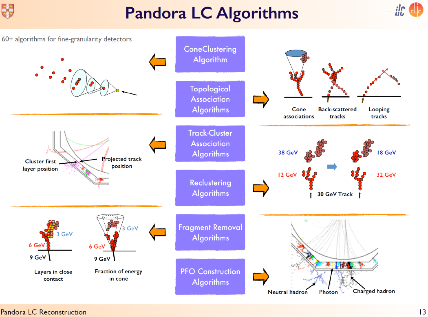
\includegraphics[width=200pt]{./Figure/EcalDetector/PandoraPFA_2.png}
		\caption[PandoraPFA のワークフロー]{PandoraPFA のワークフロー}
		\label{PandoraPFA}
	\end{center}
\end{figure}

現在のPandoraPFAのエネルギー分解能の性能を図\ref{PandoraPFA_res}に示す。カロリメータの単一ジェットに対するジェットエネルギー分解能を比較しており、このうち黒い実線はPandoraPFAを適用した時の性能である一方、赤い点線はPandoraPFAを適用していない場合の性能となっている。主に$\SI{100}{GeV}$以下の領域においてPandoraPFAを適用した場合の性能が良い分解能を示しているのがわかる。先行研究によりCalorimeterのみの場合のジェットエネルギー分解能性能は赤い点線で示された50-60\%$/\sqrt{E(\SI{}{GeV})}$である一方でPandoraPFAを適用した場合の性能は$\sim30\%/\sqrt{E(\SI{}{GeV})}$と改善しうることが示されている。しかし、その一方でカロリメータの分解能とジェット中の粒子の比から導出される理想的にPFAを適用した場合のジェットエネルギー分解能は$\sim20\%/\sqrt{E(\SI{}{GeV})}$と計算されており、PandoraPFAをさらに改善する余地があることが示唆されている。

\begin{figure}[H]
	\begin{center}
		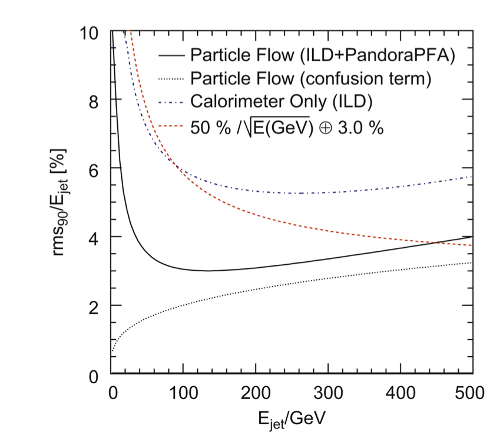
\includegraphics[width=250pt]{./Figure/EcalDetector/PFA_per.png}
		\caption[PandoraPFA を利用した場合のジェットエネルギー分解能]{PandoraPFA を利用した場合のジェットエネルギー分解能とその他の場合の比較。縦軸はエネルギー分解能を示し、小さいほど性能が良いことを示す。横軸はジェットのエネルギーである。例えば、50\%/$\sqrt{E}$という値は$\mathrm{E}_{\mathrm{jet}}$=$\SI{1}{GeV}$の時のエネルギー分解能と一致する。}
		\label{PandoraPFA_res}
	\end{center}
\end{figure}

%\subsection{PandoraPFAによるジェットエネルギー再構成性能}
%PandoraPFAを用いた際のジェットエネルギー分解能がシミュレーションデータを用いて評価された。\cite{PFATest}


%\subsection{プラスチックシンチレータ}
%シンチレータは光子検出を行うための検出器である。シンチレータに含まれる原子は光子の入射によって二次電子の放出を行い、二次電子が原子核に束縛されている電子に対して伝導体への励起を促す。しかし、二次電子によって伝導帯へと移動した電子は十分な時間が経過すると再び価電子帯へと遷移する。この際に伝導帯と価電子帯のエネルギー差に相当するシンチレーション光が発生する。通常、シンチレーション光を検出する検出器に対して波長が最適となるように、不純物をドープすることで中間準位を形成し、調整を行う。




